\chapter{Analysis and Design}
\fancyhead[R]{Analysis and Design}
\label{chap:conception}
\textit{``In this chapter, we dive into the crucial phase of our project, that of analysis and design. This is where abstract aspirations take shape, guided by a deep understanding of needs. This phase is essential for transforming identified requirements into a concrete, structured, and functional solution.''}
\pagebreak

%%%%%%%%%%%%%%%%%%%%%%%%%%%%%%%%%%%%%%%%%%%%%%%%%%%%%%%%%%%%%%%%%%%%%%%%%%%%%%%%%%%%%%%%%%
%%%%%%%%%%%%%%%%%%%%%%%%%%%%%%%%%%%%%%%%%%%%%%%%%%%%%%%%%%%%%%%%%%%%%%%%%%%%%%%%%%%%%%%%%%
%%%%%%%%%%%%%%%%%%%%%%%%%%%%%%%%%%%%%%%%%%%%%%%%%%%%%%%%%%%%%%%%%%%%%%%%%%%%%%%%%%%%%%%%%%
%%%%%%%%%%%%%%%%%%%%%%%%%%%%%%%%%%%%%%%%%%%%%%%%%%%%%%%%%%%%%%%%%%%%%%%%%%%%%%%%%%%%%%%%%%
%%%%%%%%%%%%%%%%%%%%%%%%%%%%%%%%%%%%%%%%%%%%%%%%%%%%%%%%%%%%%%%%%%%%%%%%%%%%%%%%%%%%%%%%%%
%%%%%%%%%%%%%%%%%%%%%%%%%%%%%%%%%%%%%%%%%%%%%%%%%%%%%%%%%%%%%%%%%%%%%%%%%%%%%%%%%%%%%%%%%%

\section{Analysis of the Existing System}

The current P2S compute engine is primarily a monolithic system that processes transactions collectively. It was originally designed to operate with a minimal set of input parameters, which resulted in only medium to low accuracy in fee calculations. Additionally, the system lacks the capability to distribute processing across multiple compute engines, limiting its flexibility and scalability.

To overcome these limitations, the new system is built on a stateless, event-driven architecture that supports enhanced scalability, flexibility, and accuracy where each step is stateless and we can scale on choice the stages of processing that are causing bottlenecks.
 By incorporating multiple specialized compute engines—each handling a specific component of the fee calculation—we aim to create a more modular and efficient framework.

Furthermore, in collaboration with the client, we’ve designed a comprehensive transaction data model that is ISO 20022 compliant and established a shared messaging stream.
 This stream carries a rich set of input parameters (+ 100), enabling the system to consider a wide range of factors in fee calculations and significantly improve result accuracy.


\pagebreak

%%%%%%%%%%%%%%%%%%%%%%%%%%%%%%%%%%%%%%%%%%%%%%%%%%%%%%%%%%%%%%%%%%%%%%%%%%%%%%%%%%%%%%%%%%
%%%%%%%%%%%%%%%%%%%%%%%%%%%%%%%%%%%%%%%%%%%%%%%%%%%%%%%%%%%%%%%%%%%%%%%%%%%%%%%%%%%%%%%%%%
%%%%%%%%%%%%%%%%%%%%%%%%%%%%%%%%%%%%%%%%%%%%%%%%%%%%%%%%%%%%%%%%%%%%%%%%%%%%%%%%%%%%%%%%%%
%%%%%%%%%%%%%%%%%%%%%%%%%%%%%%%%%%%%%%%%%%%%%%%%%%%%%%%%%%%%%%%%%%%%%%%%%%%%%%%%%%%%%%%%%%
%%%%%%%%%%%%%%%%%%%%%%%%%%%%%%%%%%%%%%%%%%%%%%%%%%%%%%%%%%%%%%%%%%%%%%%%%%%%%%%%%%%%%%%%%%



% \subsection{Integration Requirements}

% The system must integrate with:

% \begin{enumerate}
%     \item \textbf{Message Broker Integration}:
%     \begin{itemize}
%         \item Consume transaction messages from Kafka topics
%         \item Publish computed results to designated output topics
%         \item Implement reliable message processing patterns
%     \end{itemize}
    
%     \item \textbf{Database Integration}:
%     \begin{itemize}
%         \item Interact with PostgreSQL for configuration data
%         \item Implement connection pooling for performance
%         \item Support caching for frequently accessed data
%     \end{itemize}
    
%     \item \textbf{Monitoring Integration}:
%     \begin{itemize}
%         \item Provide performance metrics and health checks
%         \item Implement structured logging for troubleshooting
%     \end{itemize}
% \end{enumerate}

% \subsection{Success Criteria}

% The project will be successful when:

% \begin{enumerate}
%     \item \textbf{Functional Completeness}:
%     \begin{itemize}
%         \item All core computation engines are implemented and functional
%         \item Integration with payment processing infrastructure is complete
%         \item Comprehensive validation framework is operational
%     \end{itemize}
    
%     \item \textbf{Performance Achievement}:
%     \begin{itemize}
%         \item System meets required processing performance benchmarks
%         \item Scalability is demonstrated through load testing
%         \item High system availability is maintained
%     \end{itemize}
    
%     \item \textbf{Quality Validation}:
%     \begin{itemize}
%         \item Fee calculation accuracy meets business requirements
%         \item System reliability is validated through testing
%         \item Security and compliance requirements are satisfied
%     \end{itemize}
% \end{enumerate}

% \subsection{Deliverables}

% The project will produce:

% \begin{enumerate}
%     \item \textbf{P2S Compute Engines Implementation}: Production-ready computational framework with all processing engines implemented as scalable microservices.
    
%     \item \textbf{Integration Framework}: Complete message broker and database integration components supporting reliable transaction processing.
    
%     \item \textbf{Validation Framework}: Comprehensive validation system for transaction data and business rule compliance.
    
%     \item \textbf{Technical Documentation}: System architecture documentation including design specifications, integration protocols, and operational procedures.
    
%     \item \textbf{Testing Framework}: Complete testing suite including unit tests, integration tests, and performance validation tools.
% \end{enumerate}




\section{UML Diagrams}
\subsection{Class Diagram}

Uml class diagram is a visual representation of the system's classes, their attributes, methods, and relationships. It provides a high-level overview of the system's structure and serves as a blueprint for implementation.
In this section, we present the UML class diagram for the P2S Compute Engines, which illustrates the key classes and their relationships within the system.

\begin{figure}[H]
    \centering
    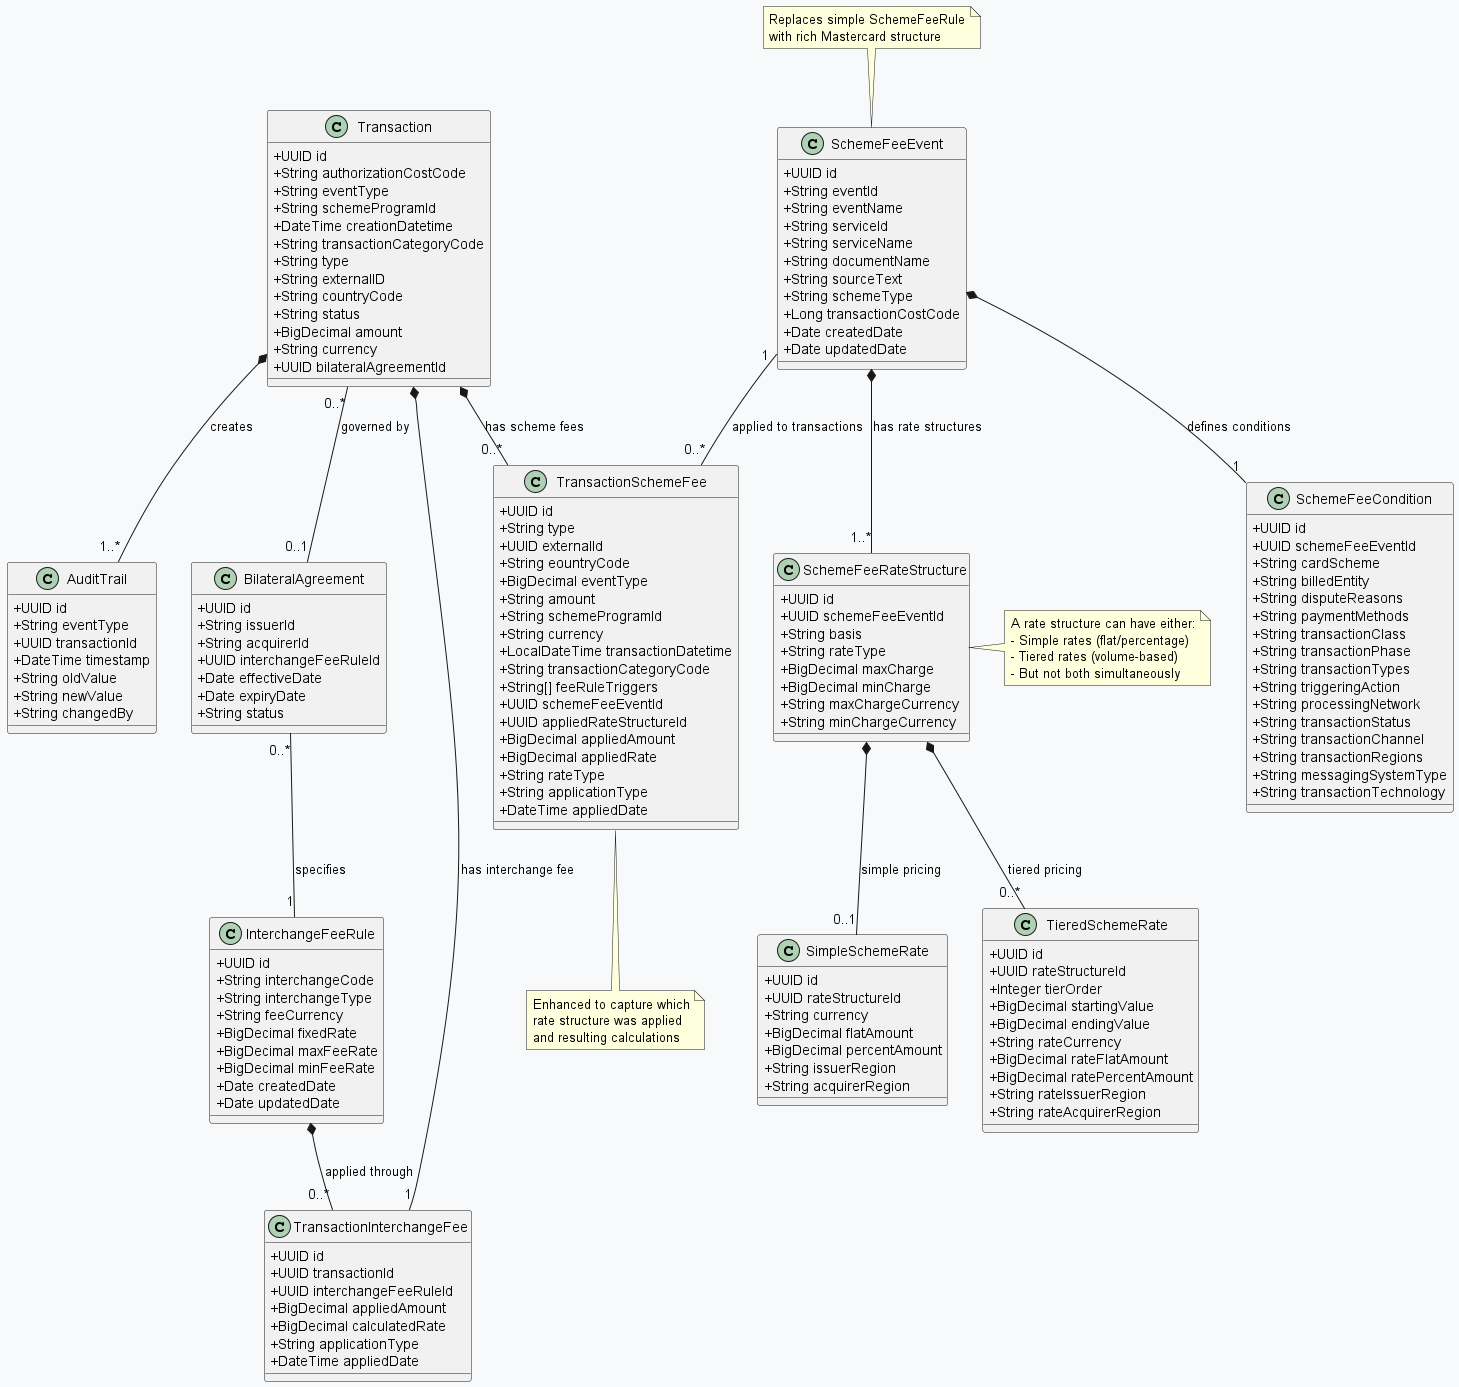
\includegraphics[width=1.05\textwidth]{out/diagrams/plantuml/in/class-diagram/class-diagram.png}
    \caption{UML Class Diagram for P2S Compute Engines}
    \label{fig:class_diagram}
\end{figure}



\subsection{Use Case Diagram}
The use case diagram provides a visual representation of the interactions between actors and the system, highlighting the key functionalities and their relationships. It serves as a high-level overview of the system's capabilities and how users will interact with it.




\begin{figure}[H]
    \centering
    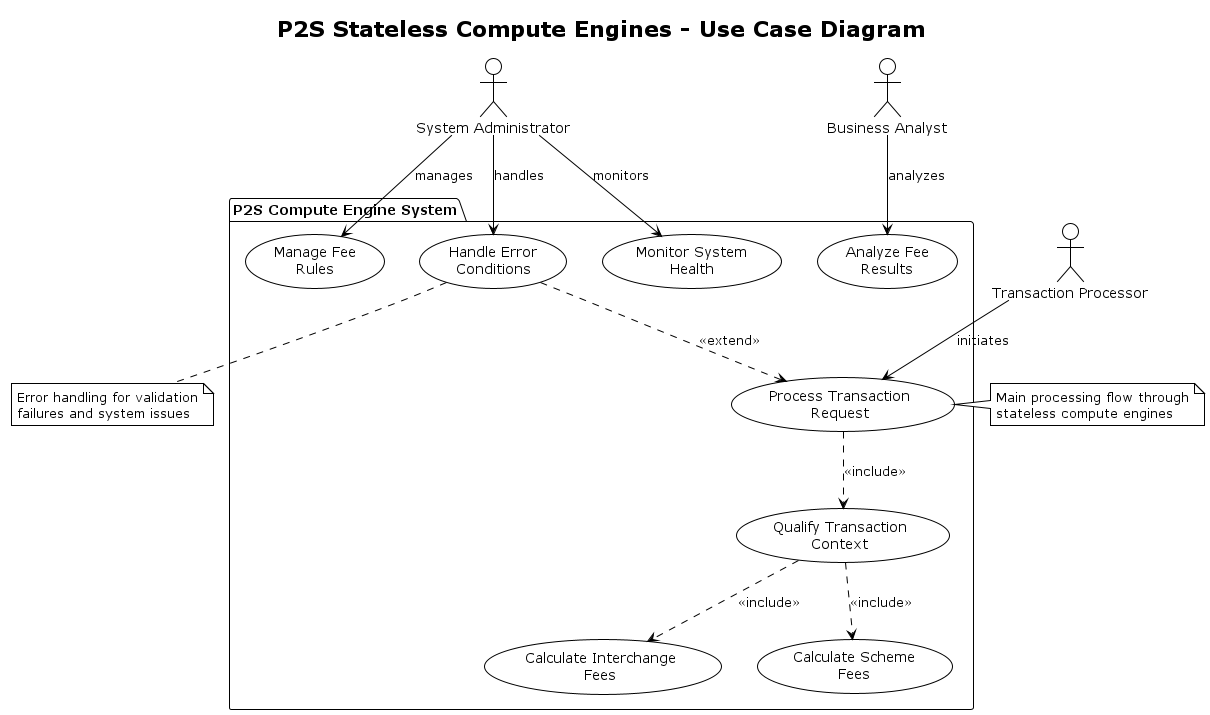
\includegraphics[width=1.05\textwidth]{out/diagrams/plantuml/in/use-case/use-case.png}
    \caption{Use Case Diagram for P2S Compute Engines}
    \label{fig:use_case_diagram}
\end{figure}



\subsection{Sequence Diagram}
The sequence diagram illustrates the flow of interactions between the components of the P2S Compute Engines during a typical transaction processing scenario. It provides a detailed view of how messages are exchanged between the various components,Context Qualification Engine, Interchange Calculation Engine, and Scheme Fees Calculation Engine.

\subsubsection{ContextQualification Sequence Diagram}



\begin{figure}[H]
    \centering
    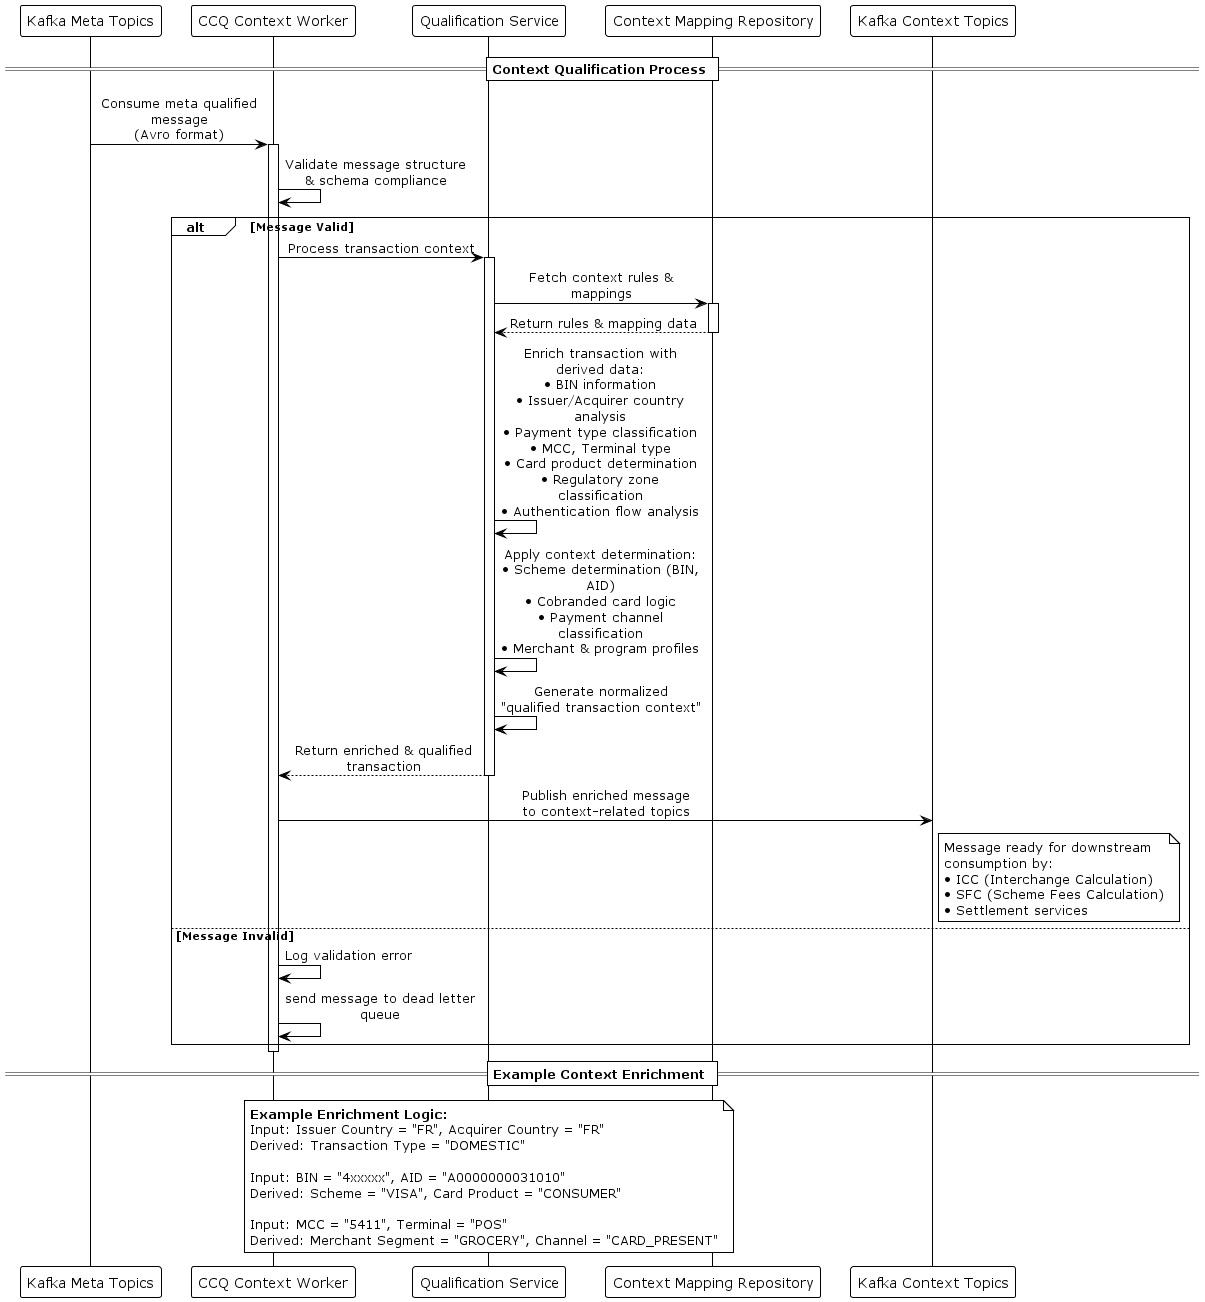
\includegraphics[width=1.05\textwidth]{out/diagrams/plantuml/in/context-sequence-diagram/P2S Context Qualification Process.png}
    \caption{Context Qualification Sequence Diagram}
    \label{fig:context_qualification_sequence}
\end{figure}   


\subsubsection{Interchange Calculation Sequence Diagram}
\begin{figure}[H]
    \centering
    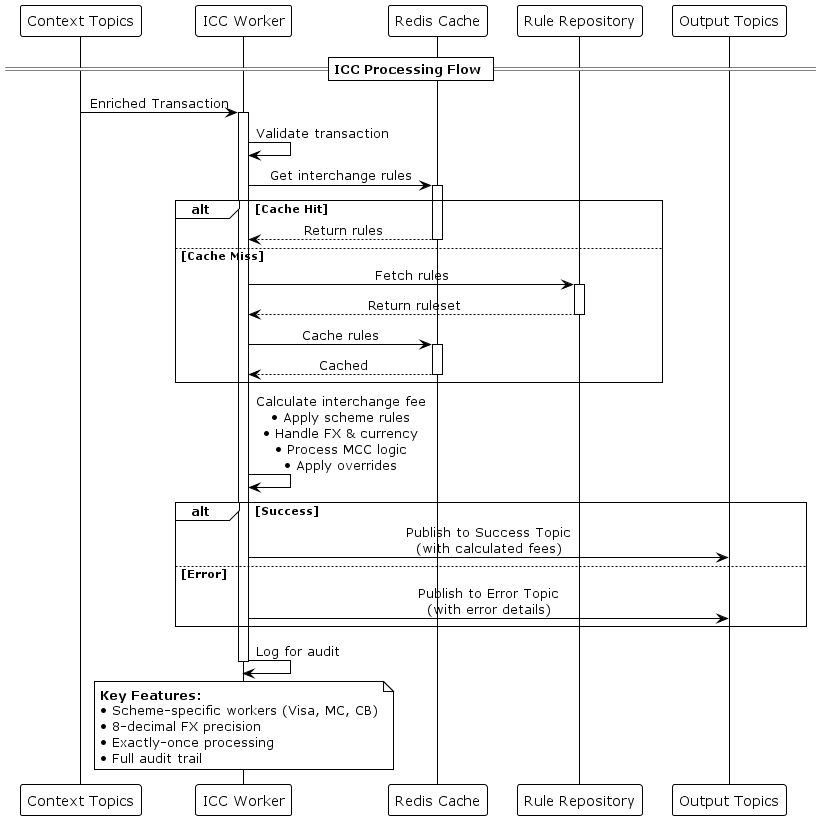
\includegraphics[width=1.05\textwidth]{out/diagrams/plantuml/in/ic-sequence/P2S Interchange Fee Calculation Process.png}
    \caption{Interchange Calculation Sequence Diagram}
    \label{fig:interchange_calculation_sequence}
\end{figure}


\subsubsection{Scheme Fees Calculation Sequence Diagram}
\begin{figure}[H]
    \centering
    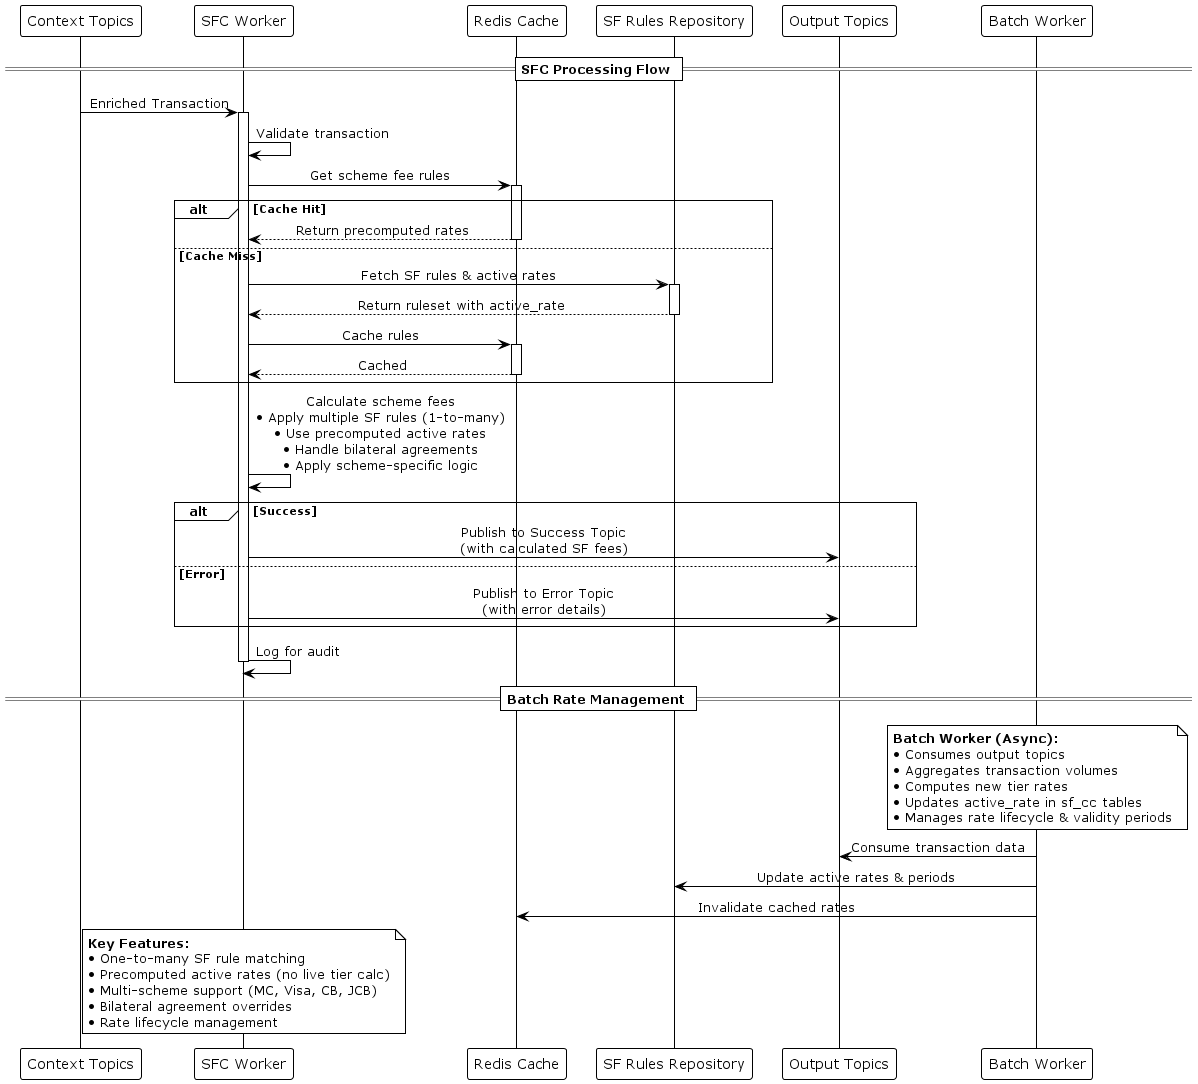
\includegraphics[width=1.05\textwidth]{out/diagrams/plantuml/in/sf-sequence/P2S Scheme Fee Calculation Process.png}
    \caption{Scheme Fees Calculation Sequence Diagram}
    \label{fig:scheme_fees_calculation_sequence}
\end{figure}

%%%%%%%%%%%%%%%%%%%%%%%%%%%%%%%%%%%%%%%%%%%%%%%%%%%%%%%%%%%%%%%%%%%%%%%%%%%%%%%%%%%%%%%%%%
%%%%%%%%%%%%%%%%%%%%%%%%%%%%%%%%%%%%%%%%%%%%%%%%%%%%%%%%%%%%%%%%%%%%%%%%%%%%%%%%%%%%%%%%%%
%%%%%%%%%%%%%%%%%%%%%%%%%%%%%%%%%%%%%%%%%%%%%%%%%%%%%%%%%%%%%%%%%%%%%%%%%%%%%%%%%%%%%%%%%%
%%%%%%%%%%%%%%%%%%%%%%%%%%%%%%%%%%%%%%%%%%%%%%%%%%%%%%%%%%%%%%%%%%%%%%%%%%%%%%%%%%%%%%%%%%
%%%%%%%%%%%%%%%%%%%%%%%%%%%%%%%%%%%%%%%%%%%%%%%%%%%%%%%%%%%%%%%%%%%%%%%%%%%%%%%%%%%%%%%%%%
%%%%%%%%%%%%%%%%%%%%%%%%%%%%%%%%%%%%%%%%%%%%%%%%%%%%%%%%%%%%%%%%%%%%%%%%%%%%%%%%%%%%%%%%%%

%%%%%%%%%%%%%%%%%%%%%%%%%%%%%%%%%%%%%%%%%%%%%%%%%%%%%%%%%%%%%%%%%%%%%%%%%%%%%%%%%%%%%%%%%%
%%%%%%%%%%%%%%%%%%%%%%%%%%%%%%%%%%%%%%%%%%%%%%%%%%%%%%%%%%%%%%%%%%%%%%%%%%%%%%%%%%%%%%%%%%
%%%%%%%%%%%%%%%%%%%%%%%%%%%%%%%%%%%%%%%%%%%%%%%%%%%%%%%%%%%%%%%%%%%%%%%%%%%%%%%%%%%%%%%%%%
%%%%%%%%%%%%%%%%%%%%%%%%%%%%%%%%%%%%%%%%%%%%%%%%%%%%%%%%%%%%%%%%%%%%%%%%%%%%%%%%%%%%%%%%%%
%%%%%%%%%%%%%%%%%%%%%%%%%%%%%%%%%%%%%%%%%%%%%%%%%%%%%%%%%%%%%%%%%%%%%%%%%%%%%%%%%%%%%%%%%%
%%%%%%%%%%%%%%%%%%%%%%%%%%%%%%%%%%%%%%%%%%%%%%%%%%%%%%%%%%%%%%%%%%%%%%%%%%%%%%%%%%%%%%%%%%

\section{Conclusion}

Conclusion here